El dispositivo de ramificación óptico bidireccional utilizado en PONs punto a multipunto (P2MP), que tiene una entrada desde el puerto F1 y múltiples puertos de salida, se denomina divisor óptico o simplemente divisor (splitter, en inglés). Los divisores se consideran pasivos al no precisar de una fuente de energía externa, salvo el haz de luz incidente. Son de banda ancha y solo agregan pérdida, principalmente debido al hecho de que dividen la potencia de entrada (de forma descendente). Esta pérdida, conocida como pérdida de divisor o relación de división, se expresa normalmente en dB y depende principalmente de su número de puertos de salida, como se muestra en el cuadro~\tableref{table:Splitter_losses}.

La señal óptica (descendente) de entrada se divide en partes iguales en cascada o ramificaciones; por ejemplo, un divisor 1×2 solo tiene dos ramificaciones o una división que soporta una pérdida de 3 dB (50\% de luz en cada ruta). En un divisor 1×4, se agregan otras dos ramificaciones a cada ruta de la división 1×2 original, añadiendo otros 3 dB, para una pérdida total de 6 dB. En un divisor 1×8, se añaden dos ramificaciones más o división 1×2 a cada ruta de la división 1×4 original, añadiendo nuevamente otra pérdida de 3 dB para una pérdida total de 9 dB. Un divisor 1×16 soportará entonces una pérdida de 12 dB y un divisor 1×32 tendrá una pérdida mínima de 15 dB, sin contar las pérdidas adicionales debidas a conexiones e imperfecciones (normalmente se añade 1 dB a la pérdida de división original); por tanto, un divisor 1×32 tendrá normalmente una pérdida de 16 dB.

Las \textbf{PONs} utilizan cada uno de los puertos de salida a F2, lo que permite que múltiples usuarios compartan una misma fibra óptica y, en consecuencia, el ancho de banda. En la dirección ascendente, las señales ópticas se combinan desde diversos ONTs en una fibra única (F1).

Cabe señalar, que contrariamente a lo que cabría esperar, el divisor añade aproximadamente la misma pérdida; en ambos sentidos, incluso para laseñal transmitida en dirección ascendente.

%% \noindent
\begin{center}
 
%%\begin{spacing}{1}  
\begin{table}[H]  %%\centering

    \setlength\arrayrulewidth{1.5pt}
    \arrayrulecolor{white}
    \def\clinecolor{\hhline{|>{\arrayrulecolor{white}}-%
    >{\arrayrulecolor{white}}|-|-|}}
\resizebox{0.98 \textwidth}{!}{% 
       
\begin{tabularx}{1 \textwidth}%
    {|
    >{\columncolor{white} \centering\arraybackslash}m{0.25\textwidth}
     |
    >{\columncolor{white} \centering\arraybackslash}m{0.70\textwidth}
     |
    }
    \rowcolor{HeadersColor} \thead{Número de puertos} & \thead{Pérdida de divisor (dB) (excluidas conexiones y pérdida \\ de divisor excesiva}  \\    
    \hhline{|-|-|}
    \rowcolor{gray!20} 2 & 3 \\
    \hhline{|-|-|}
    \rowcolor{gray!20} 4 & 6 \\ 
    \hhline{|-|-|}
    \rowcolor{gray!20} 8 & 9 \\     
    \hhline{|-|-|}
    \rowcolor{gray!20} 16 & 12 \\  
    \hhline{|-|-|}
    \rowcolor{gray!20} 32 & 15 \\   
    \hhline{|-|-|}
    \rowcolor{gray!20} 64 & 18 \\                  
    \end{tabularx}}
	\caption{\footnotesize{Pérdida de divisor}}
	\label{table:Splitter_losses}
\end{table}
%%\end{spacing}

\end{center}




\begin{wrapfigure}[12]{l}{0.55\textwidth}
  \begin{center}
   	\includegraphics[width=0.55\textwidth]{./img/punto5/Divisor-de-guía-de-onda-planar-PLC.jpg}	
   	\caption{Divisor de guía de onda planar (PLC)}
	\label{fig:Planar_wave_guide}
  \end{center}  
\end{wrapfigure}


En una red FTTH, puede haber un divisor o varios divisores en cascada, en función de la topología. La recomendación G.984 de la ITU-T permite relaciones de división de hasta 31, mientras que la recomendación G.984.6 amplía la relación hasta 64. Independientemente de la topología, el divisor debe satisfacer el presupuesto de pérdida óptica previsto. \\

\vfill

\clearpage


Los divisores pueden ser confeccionados en diferentes formas y tamaños en función de la tecnología básica utilizada. Los tipos más comunes son los de tipo encapsulado, denominados PLC (normalmente para elevadas relaciones de división) y los confeccionados mediante fusiones múltiples (FBT) (normalmente para bajos niveles de división). Ambos tipos se fabrican para su montaje en conjuntos de caja-bandeja. En la figura~\figref{fig:FBT_splitter} muestra las dos tecnologías.



\begin{figure}[H]
	\centering
	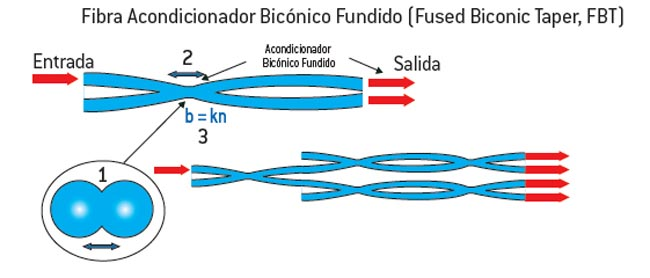
\includegraphics[width=0.86\textwidth]{./img/punto5/Divisor-FBT.jpg}
	\caption{Divisor FBT}
	\label{fig:FBT_splitter}
\end{figure}



